\chapter{Análisis del problema}\label{ch:analisis-del-problema}

Para realizar cualquier proyecto de Ingeniería del Software es necesario llevar a cabo un análisis del problema,
en el que se definen los requisitos del sistema, se describen los actores que interactúan con el sistema y se
realizan los diagramas de caso de uso. El objetivo es conseguir un producto que cumpla con los requisitos y
necesidades que requiere el cliente.

\section{Ingeniería de requisitos}\label{sec:ingenieria-de-requisitos}

La ingeniería de requisitos consiste en la definición delos requisitos del sistema, es decir, las características
que debe tener el sistema para que sea aceptado por el cliente. Durante esta fase se llevan a cabo una serie
de actividades que permiten obtener un producto de calidad:

\begin{itemize}
    \item \textbf{Identificación de requisitos}: se recopila información sobre el sistema y se identifican
    las necesidades de usuarios, organizaciones y partes interesadas.
    \item \textbf{Análisis de requisitos}: se realiza una descripción detallada de los requisitos del sistema,
    se definen los casos de uso y se identifican los actores que interactúan con el sistema así como los
    requisitos funcionales y no funcionales.
    \item \textbf{Viabilidad del sistema}: se comprueba que el sistema es viable, es decir, que se pueda
    desarrollar cumpliendo los requisitos y se comprueba que estos sean consistentes, completos y no contradictorios.
\end{itemize}

\newpage

\subsection{Requisitos funcionales}\label{subsec:requisitos-funcionales}

Los requisitos funcionales son aquellos que definen las funciones que debe realizar el sistema. Describen la
interacción entre el sistema y el usuario, es decir, lo que el usuario puede hacer con el sistema. En este caso,
a pesar de tener como actores a los usuarios y a la organización, los requisitos funcionales se centran en
las funciones que puede realizar la organización ya que es la que va a utilizar el sistema que se va a desarrollar.
Los requisitos referidos a los usuarios se describen en la aplicación móvil que desarrollará mi compañero de
trabajo.

\begin{itemize}
    \item \textbf{RF-1.} Gestión de la organización
    \begin{itemize}
        \item \textbf{RF-1.1.} Alta de organización
        \item \textbf{RF-1.2.} Subir foto de perfil
        \item \textbf{RF-1.3.} Modificar información de la organización
        \item \textbf{RF-1.4.} Recuperar contraseña
        \item \textbf{RF-1.5.} Desactivar cuenta
        \item \textbf{RF-1.6.} Activar cuenta
    \end{itemize}
    \item \textbf{RF-2.} Gestión de animales
    \begin{itemize}
        \item \textbf{RF-2.1.} Alta de animales
        \item \textbf{RF-2.2.} Baja de animales
        \item \textbf{RF-2.3.} Modificación de la información de los animales
        \item \textbf{RF-2.4.} Subir fotos de los animales
        \item \textbf{RF-2.5.} Eliminar fotos de los animales
    \end{itemize}
    \item \textbf{RF-3.} Gestión de peticiones
    \begin{itemize}
        \item \textbf{RF-3.1.} Actualizar estado
        \item \textbf{RF-3.2.} Aprobar información del usuario
        \item \textbf{RF-3.3.} Rechazar información del usuario
        \item \textbf{RF-3.4.} Aprobar documentación del usuario
        \item \textbf{RF-3.5.} Rechazar documentación del usuario
        \item \textbf{RF-3.6.} Aprobar petición
        \item \textbf{RF-3.7.} Rechazar petición
    \end{itemize}
\end{itemize}

\subsection{Requisitos no funcionales}\label{subsec:requisitos-no-funcionales}

Los requisitos no funcionales son aquellos que describen las restricciones o características que debe cumplir el
sistema. A diferencia de los funcionales, estos requisitos no se centran en las funciones que debe realizar el sistema.

\begin{table}[H]
    \centering
    \begin {tabular} {| l | l |}
        \hline
        \textbf {RFN-1}
        & \underline{Usabilidad} \\
        & \tabitem El sistema debe ser fácil de usar \\
        & \tabitem El sistema debe ser intuitivo \\
        \hline

        \textbf {RFN-2}
        & \underline{Seguridad} \\
        & \tabitem El sistema debe tener un sistema de autenticación \\
        & \tabitem El sistema debe tener un sistema de verificación de la identidad \\
        & \tabitem El sistema debe proteger la información de los usuarios y organizaciones \\
        \hline

        \textbf {RFN-3}
        & \underline{Fiabilidad} \\
        & \tabitem El sistema debe ser resistente a fallos \\
        & \tabitem El sistema debe ser resistente a ataques externos \\
        \hline

        \textbf {RFN-4}
        & \underline{Rendimiento} \\
        & \tabitem El sistema debe ser rápido \\
        & \tabitem El sistema debe ser escalable \\
        \hline

        \textbf {RFN-5}
        & \underline{Eficiencia} \\
        & \tabitem El sistema debe ser eficiente en el uso de los recursos \\
        & \tabitem El sistema debe ser capaz de soportar un gran número de usuarios \\
        & \tabitem El sistema debe ser capaz de soportar un gran número de peticiones \\
        & \tabitem El sistema debe ser capaz de soportar un gran número de animales \\
        & \tabitem El sistema debe ser capaz de soportar un gran número de imágenes \\
        \hline

        \textbf {RFN-6}
        & \underline{Compatibilidad} \\
        & \tabitem El sistema debe ser compatible con los navegadores más utilizados \\
        & \tabitem El sistema debe ser compatible con los dispositivos más utilizados \\
        \hline

        \textbf {RFN-7}
        & \underline{Disponibilidad} \\
        & \tabitem El sistema debe estar disponible el mayor tiempo posible \\
        \hline

        \textbf {RFN-8}
        & \underline{Mantenibilidad} \\
        & \tabitem El sistema debe ser fácil de mantener \\
        & \tabitem El sistema debe ser fácil de actualizar \\
        \hline

        \textbf {RFN-9}
        & \underline{Ética} \\
        & \tabitem El sistema debe cumplir con la normativa vigente de protección de datos \\
        & \tabitem El sistema debe cumplir con la normativa vigente de protección de animales \\
        \hline

    \end {tabular}
    \caption {Requisitos no funcionales}
    \label {tab:requisitos-no-funcionales}
\end {table}

\newpage

\subsection{Requisitos de información}\label{subsec:requisitos-de-informacion}

Los requisitos de información son aquellos que describen la información que debe almacenar el sistema (aplicación web).

\begin{table}[H]
    \centering
    \begin {tabular} {| l | l |}
        \hline
        \textbf {RI-1}
        & \underline{Organizaciones} \\
        & \tabitem Información para el registro en la aplicación \\
        & \tabitem Información de contacto: nombre, teléfono, email, foto de perfil, dirección\ldots \\
        & \textbf{Requisitos funcionales:} RF-2. \\
        \hline

        \textbf {RI-2}
        & \underline{Usuarios} \\
        & \tabitem Información para el registro en la aplicación \\
        & \tabitem Información de contacto: nombre, teléfono, email, foto de perfil, dirección\ldots \\
        & \tabitem Información de las mascotas guardadas en favoritos \\
        & \tabitem Información de las peticiones realizadas \\
        \hline

        \textbf {RI-3}
        & \underline{Animales} \\
        & \tabitem Información del animal: nombre, raza, edad, sexo, tamaño\ldots \\
        & \tabitem Imágenes del animal \\
        & \textbf{Requisitos funcionales:} RF-1. \\
        \hline

        \textbf {RI-4}
        & \underline{Peticiones} \\
        & \tabitem Información de la petición: animal, descripción, fecha de creación, estado\ldots \\
        & \textbf{Requisitos funcionales:} RF-3. \\
        \hline

    \end {tabular}
    \caption {Requisitos de información}
    \label {tab:requisitos-informacion}
\end {table}

\newpage

\section{Descripción de actores}\label{sec:descripcion-de-actores}

Los actores son los elementos que interactúan con el sistema. En este caso, los actores son las organizaciones y los usuarios.
También existe un actor \textbf{admin} que es el encargado de gestionar la aplicación pero no interactúa con ella directamente.
No se ha considerado como un actor externo ya que coincide con el propio desarrollador del proyecto y se obvia que
tiene todos los privilegios sobre la aplicación y la base de datos y por tanto puede realizar cualquier acción.

En la siguiente tabla se describe únicamente la información relevante a la organización ya que el usuario no
pertenece a la aplicación web, sino que participa en la aplicación móvil y no tiene información relevante para esta
documentación.


\subsection{Organización}\label{subsec:organizacion}

\begin{table}[H]
\begin{center}
    \begin{adjustbox}{width=\textwidth}
    \begin{tabular}{ | l | l | l | l | c | c | }
        \hline
        \textbf{Actor} & \multicolumn{4}{l|}{Organización} & \cellcolor{gray!50} \textbf{ACT-1}\\
        \hline
        \textbf{Descripción} & \multicolumn{5}{p{0.9\linewidth}|}{Representa a una
        organización que se registra en la aplicación (asociación, protectora, refugio\ldots).} \\
        \hline
        \textbf{Características} & \multicolumn{5}{p{0.5\linewidth}|}{Está registrada
        en el sistema y por tanto puede publicar animales y gestionar la información de los animales y las peticiones.} \\
        \hline
        \textbf{Relaciones} & \multicolumn{5}{p{0.5\linewidth}|}{ } \\
        \hline
        \textbf{Referencias} & \multicolumn{5}{p{0.5\linewidth}|}{CU-1.1, CU-1.2, CU-1.3, CU-1.4, CU-1.5, CU-1.6,
        CU-2.1, CU-2.2, CU-2.3, CU-2.4, CU-2.5, CU-3.1, CU-3.2, CU-3.3, CU-3.4, CU-3.5, CU-3.6, CU-3.7 } \\
        \hline
        \textbf{Autor} & \multicolumn{1}{p{0.25\linewidth}|}{Manuel Ángel Rodríguez Segura} & \textbf{Fecha} &
        08-04-2023     & \textbf{Versión}                                                      & 1.0\\
        \hline
    \end{tabular}
    \end{adjustbox}
    \caption{Actor: Organización}
    \label{tab:organizacion}
\end{center}
\end{table}

\newpage

\section{Diagramas de Caso de Uso}\label{sec:diagramas-de-caso-de-uso}

Los diagramas de caso de uso son una representación gráfica que nos permite visualizar los actores y las acciones que
pueden realizar sobre el sistema. En el desarrollo de software son una herramienta muy útil para la comunicación entre
el cliente y el desarrollador ya que permiten mostrar de forma sencilla las funcionalidades del sistema. \\

Para la realización de los diagramas de caso de uso se ha utilizado la herramienta de Google \textbf{draw.io}.
A continuación se muestran los diferentes diagramas involucrados en el sistema:

\subsection{Gestión de organización}\label{subsec:gestion-de-organizacion}

\begin{figure}[H]
    \centering
    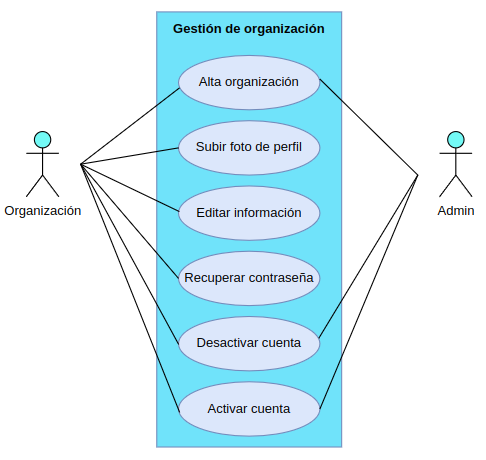
\includegraphics[width=0.8\textwidth]{imgs/gestion-organizacion}
    \caption{Gestión de organización}
    \label{fig:diagrama-caso-uso-gestion-organizacion}
\end{figure}

\subsubsection{Caso de Uso 1.1: Alta organización}\label{subsubsec:alta-organizacion}

\begin{table}[H]
    \begin{center}
        \begin{adjustbox}{width=\textwidth}
            \begin{tabular}{ | l | l | l | l | c | c | }
                \hline
                \textbf{Caso de uso} & \multicolumn{4}{l|}{Alta organización} & \cellcolor{gray!50} \textbf{CU-1.1}\\
                \hline
                \textbf{Actores} & \multicolumn{5}{p{0.5\linewidth}|}{Organización, admin} \\
                \hline
                \textbf{Tipo} & \multicolumn{5}{l|}{Primario y esencial} \\
                \hline
                \textbf{Referencias} & \multicolumn{3}{l|}{RF-1.1} & \multicolumn{2}{l|}{ }\\
                \hline
                \textbf{Precondición} & \multicolumn{5}{l|}{La organización no puede estar registrada previamente} \\
                \hline
                \textbf{Postcondición} & \multicolumn{5}{l|}{La organización es registrada y puede usar la aplicación en su totalidad} \\
                \hline
                \textbf{Autor} & \multicolumn{1}{p{0.25\linewidth}|}{Manuel Ángel Rodríguez Segura} & \textbf{Fecha} &
                08-04-2023     & \textbf{Versión}                                                      & 1.0\\
                \hline
            \end{tabular}
        \end{adjustbox}
        \caption{CU-1.1: Alta organización}
        \label{tab:alta-organizacion}
    \end{center}
\end{table}

\begin{table}[H]
    \centering
    \begin{tabularx}{\textwidth}{@{} |L |@{}} \hline
        \rowcolor{gray!50}
        \textbf{Propósito} \\
        \hline
        Permite a una organización registrarse en el sistema. \\
        \hline
    \end{tabularx}
\end{table}

\begin{table}[H]
    \centering
    \begin{tabularx}{\textwidth}{@{} |L |@{}} \hline
        \rowcolor{gray!50}
        \textbf{Resumen} \\
        \hline
        Permite a una organización registrarse en el sistema y acceder a todas las funcionalidades de la aplicación. \\
        \hline
    \end{tabularx}
\end{table}

\subsubsection{Caso de Uso 1.2: Subir foto de perfil}\label{subsubsec:subir-foto-perfil}

\begin{table}[H]
    \begin{center}
        \begin{adjustbox}{width=\textwidth}
            \begin{tabular}{ | l | l | l | l | c | c | }
                \hline
                \textbf{Caso de uso} & \multicolumn{4}{l|}{Subir foto de perfil} & \cellcolor{gray!50} \textbf{CU-1.2}\\
                \hline
                \textbf{Actores} & \multicolumn{5}{p{0.5\linewidth}|}{Organización} \\
                \hline
                \textbf{Tipo} & \multicolumn{5}{l|}{Primario y esencial} \\
                \hline
                \textbf{Referencias} & \multicolumn{3}{l|}{RF-1.2} & \multicolumn{2}{l|}{ }\\
                \hline
                \textbf{Precondición} & \multicolumn{5}{l|}{La organización debe estar registrada previamente} \\
                \hline
                \textbf{Postcondición} & \multicolumn{5}{l|}{La organización tiene una foto de perfil} \\
                \hline
                \textbf{Autor} & \multicolumn{1}{p{0.25\linewidth}|}{Manuel Ángel Rodríguez Segura} & \textbf{Fecha} &
                08-04-2023     & \textbf{Versión}                                                      & 1.0\\
                \hline
            \end{tabular}
        \end{adjustbox}
        \caption{CU-1.2: Subir foto de perfil}
        \label{tab:subir-foto-perfil}
    \end{center}
\end{table}

\begin{table}[H]
    \centering
    \begin{tabularx}{\textwidth}{@{} |L |@{}} \hline
        \rowcolor{gray!50}
        \textbf{Propósito} \\
        \hline
        Permite a una organización subir una foto de perfil. \\
        \hline
    \end{tabularx}
\end{table}

\begin{table}[H]
    \centering
    \begin{tabularx}{\textwidth}{@{} |L |@{}} \hline
        \rowcolor{gray!50}
        \textbf{Resumen} \\
        \hline
        Permite a una organización subir y actualizar su foto de perfil. \\
        \hline
    \end{tabularx}
\end{table}

\subsubsection{Caso de Uso 1.3: Editar información}\label{subsubsec:editar-informacion}

\begin{table}[H]
    \begin{center}
        \begin{adjustbox}{width=\textwidth}
            \begin{tabular}{ | l | l | l | l | c | c | }
                \hline
                \textbf{Caso de uso} & \multicolumn{4}{l|}{Editar información} & \cellcolor{gray!50} \textbf{CU-1.3}\\
                \hline
                \textbf{Actores} & \multicolumn{5}{p{0.5\linewidth}|}{Organización} \\
                \hline
                \textbf{Tipo} & \multicolumn{5}{l|}{Primario y esencial} \\
                \hline
                \textbf{Referencias} & \multicolumn{3}{l|}{RF-1.3} & \multicolumn{2}{l|}{ }\\
                \hline
                \textbf{Precondición} & \multicolumn{5}{l|}{La organización debe estar registrada previamente} \\
                \hline
                \textbf{Postcondición} & \multicolumn{5}{l|}{La organización tiene una foto de perfil} \\
                \hline
                \textbf{Autor} & \multicolumn{1}{p{0.25\linewidth}|}{Manuel Ángel Rodríguez Segura} & \textbf{Fecha} &
                08-04-2023     & \textbf{Versión}                                                      & 1.0\\
                \hline
            \end{tabular}
        \end{adjustbox}
        \caption{CU-1.3: Editar información}
        \label{tab:editar-organizacion}
    \end{center}
\end{table}

\begin{table}[H]
    \centering
    \begin{tabularx}{\textwidth}{@{} |L |@{}} \hline
        \rowcolor{gray!50}
        \textbf{Propósito} \\
        \hline
        Permite a una organización editar su información. \\
        \hline
    \end{tabularx}
\end{table}

\begin{table}[H]
    \centering
    \begin{tabularx}{\textwidth}{@{} |L |@{}} \hline
        \rowcolor{gray!50}
        \textbf{Resumen} \\
        \hline
        Permite a una organización editar su información (teléfono, dirección, etc.). \\
        \hline
    \end{tabularx}
\end{table}

\subsubsection{Caso de Uso 1.4: Recuperar contraseña}\label{subsubsec:recuperar-contrasena}

\begin{table}[H]
    \begin{center}
        \begin{adjustbox}{width=\textwidth}
            \begin{tabular}{ | l | l | l | l | c | c | }
                \hline
                \textbf{Caso de uso} & \multicolumn{4}{l|}{Recuperar contraseña} & \cellcolor{gray!50} \textbf{CU-1.4}\\
                \hline
                \textbf{Actores} & \multicolumn{5}{p{0.5\linewidth}|}{Organización} \\
                \hline
                \textbf{Tipo} & \multicolumn{5}{l|}{Primario y esencial} \\
                \hline
                \textbf{Referencias} & \multicolumn{3}{l|}{RF-1.4} & \multicolumn{2}{l|}{ }\\
                \hline
                \textbf{Precondición} & \multicolumn{5}{l|}{La organización debe estar registrada previamente} \\
                \hline
                \textbf{Postcondición} & \multicolumn{5}{l|}{La organización recupera su contraseña} \\
                \hline
                \textbf{Autor} & \multicolumn{1}{p{0.25\linewidth}|}{Manuel Ángel Rodríguez Segura} & \textbf{Fecha} &
                08-04-2023     & \textbf{Versión}                                                      & 1.0\\
                \hline
            \end{tabular}
        \end{adjustbox}
        \caption{CU-1.4: Recuperar contraseña}
        \label{tab:recuperar-contrasena}
    \end{center}
\end{table}

\begin{table}[H]
    \centering
    \begin{tabularx}{\textwidth}{@{} |L |@{}} \hline
        \rowcolor{gray!50}
        \textbf{Propósito} \\
        \hline
        Permite a una organización recuperar su contraseña por medio de un correo electrónico. \\
        \hline
    \end{tabularx}
\end{table}

\begin{table}[H]
    \centering
    \begin{tabularx}{\textwidth}{@{} |L |@{}} \hline
        \rowcolor{gray!50}
        \textbf{Resumen} \\
        \hline
        Permite a una organización recuperar su contraseña por medio de un correo electrónico. \\
        \hline
    \end{tabularx}
\end{table}

\subsubsection{Caso de Uso 1.5: Editar información}\label{subsubsec:editar-informacion-org}

\begin{table}[H]
    \begin{center}
        \begin{adjustbox}{width=\textwidth}
            \begin{tabular}{ | l | l | l | l | c | c | }
                \hline
                \textbf{Caso de uso} & \multicolumn{4}{l|}{Desactivar cuenta} & \cellcolor{gray!50} \textbf{CU-1.5}\\
                \hline
                \textbf{Actores} & \multicolumn{5}{p{0.5\linewidth}|}{Organización} \\
                \hline
                \textbf{Tipo} & \multicolumn{5}{l|}{Primario y esencial} \\
                \hline
                \textbf{Referencias} & \multicolumn{3}{l|}{RF-1.5} & \multicolumn{2}{l|}{ }\\
                \hline
                \textbf{Precondición} & \multicolumn{5}{l|}{La organización debe estar registrada previamente} \\
                \hline
                \textbf{Postcondición} & \multicolumn{5}{l|}{La organización desactiva su cuenta} \\
                \hline
                \textbf{Autor} & \multicolumn{1}{p{0.25\linewidth}|}{Manuel Ángel Rodríguez Segura} & \textbf{Fecha} &
                08-04-2023     & \textbf{Versión}                                                      & 1.0\\
                \hline
            \end{tabular}
        \end{adjustbox}
        \caption{CU-1.5: Desactivar cuenta}
        \label{tab:desactivar-cuenta}
    \end{center}
\end{table}

\begin{table}[H]
    \centering
    \begin{tabularx}{\textwidth}{@{} |L |@{}} \hline
        \rowcolor{gray!50}
        \textbf{Propósito} \\
        \hline
        Permite a una organización desactivar su cuenta. \\
        \hline
    \end{tabularx}
\end{table}

\begin{table}[H]
    \centering
    \begin{tabularx}{\textwidth}{@{} |L |@{}} \hline
        \rowcolor{gray!50}
        \textbf{Resumen} \\
        \hline
        Permite a una organización desactivar su cuenta temporalmente y reactivarla cuando lo desee. Mientras
        la cuenta esté desactivada, no podrá acceder a la aplicación. \\
        \hline
    \end{tabularx}
\end{table}

\subsubsection{Caso de Uso 1.6: Activar cuenta}\label{subsubsec:activar-cuenta-org}

\begin{table}[H]
    \begin{center}
        \begin{adjustbox}{width=\textwidth}
            \begin{tabular}{ | l | l | l | l | c | c | }
                \hline
                \textbf{Caso de uso} & \multicolumn{4}{l|}{Activar cuenta} & \cellcolor{gray!50} \textbf{CU-1.6}\\
                \hline
                \textbf{Actores} & \multicolumn{5}{p{0.5\linewidth}|}{Organización} \\
                \hline
                \textbf{Tipo} & \multicolumn{5}{l|}{Primario y esencial} \\
                \hline
                \textbf{Referencias} & \multicolumn{3}{l|}{RF-1.6} & \multicolumn{2}{l|}{ }\\
                \hline
                \textbf{Precondición} & \multicolumn{5}{l|}{La organización debe estar desactivada previamente} \\
                \hline
                \textbf{Postcondición} & \multicolumn{5}{l|}{La organización activa su cuenta} \\
                \hline
                \textbf{Autor} & \multicolumn{1}{p{0.25\linewidth}|}{Manuel Ángel Rodríguez Segura} & \textbf{Fecha} &
                08-04-2023     & \textbf{Versión}                                                      & 1.0\\
                \hline
            \end{tabular}
        \end{adjustbox}
        \caption{CU-1.6: Activar cuenta}
        \label{tab:activar-cuenta}
    \end{center}
\end{table}

\begin{table}[H]
    \centering
    \begin{tabularx}{\textwidth}{@{} |L |@{}} \hline
        \rowcolor{gray!50}
        \textbf{Propósito} \\
        \hline
        Permite a una organización activar su cuenta. \\
        \hline
    \end{tabularx}
\end{table}

\begin{table}[H]
    \centering
    \begin{tabularx}{\textwidth}{@{} |L |@{}} \hline
        \rowcolor{gray!50}
        \textbf{Resumen} \\
        \hline
        Permite a una organización activar su cuenta y acceder a la aplicación de nuevo. \\
        \hline
    \end{tabularx}
\end{table}

\subsection{Gestión de animales}\label{subsec:gestion-de-animales}

\begin{figure}[H]
    \centering
    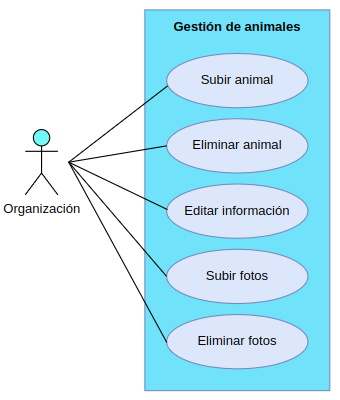
\includegraphics[width=0.8\textwidth]{imgs/gestion-animales}
    \caption{Gestión de animales}
    \label{fig:diagrama-caso-uso-gestion-animales}
\end{figure}

\subsubsection{Caso de Uso 2.1: Crear animal}\label{subsubsec:crear-animal}

\begin{table}[H]
    \begin{center}
        \begin{adjustbox}{width=\textwidth}
            \begin{tabular}{ | l | l | l | l | c | c | }
                \hline
                \textbf{Caso de uso} & \multicolumn{4}{l|}{Subir animal} & \cellcolor{gray!50} \textbf{CU-1.7}\\
                \hline
                \textbf{Actores} & \multicolumn{5}{p{0.5\linewidth}|}{Organización} \\
                \hline
                \textbf{Tipo} & \multicolumn{5}{l|}{Primario y esencial} \\
                \hline
                \textbf{Referencias} & \multicolumn{3}{l|}{RF-2.1} & \multicolumn{2}{l|}{ }\\
                \hline
                \textbf{Precondición} & \multicolumn{5}{l|}{La organización debe estar registrada previamente} \\
                \hline
                \textbf{Postcondición} & \multicolumn{5}{l|}{La organización sube un animal a la plataforma} \\
                \hline
                \textbf{Autor} & \multicolumn{1}{p{0.25\linewidth}|}{Manuel Ángel Rodríguez Segura} & \textbf{Fecha} &
                08-04-2023     & \textbf{Versión}                                                      & 1.0\\
                \hline
            \end{tabular}
        \end{adjustbox}
        \caption{CU-2.1: Subir animal}
        \label{tab:subir-animal}
    \end{center}
\end{table}

\begin{table}[H]
    \centering
    \begin{tabularx}{\textwidth}{@{} |L |@{}} \hline
        \rowcolor{gray!50}
        \textbf{Propósito} \\
        \hline
        Permite a una organización subir un animal a la plataforma. \\
        \hline
    \end{tabularx}
\end{table}

\begin{table}[H]
    \centering
    \begin{tabularx}{\textwidth}{@{} |L |@{}} \hline
        \rowcolor{gray!50}
        \textbf{Resumen} \\
        \hline
        Permite a una organización subir un animal a la aplicación para que pueda ser visto por los usuarios y adoptado
        por ellos. \\
        \hline
    \end{tabularx}
\end{table}

\subsubsection{Caso de Uso 2.2: Eliminar animal}\label{subsubsec:eliminar-animal}

\begin{table}[H]
    \begin{center}
        \begin{adjustbox}{width=\textwidth}
            \begin{tabular}{ | l | l | l | l | c | c | }
                \hline
                \textbf{Caso de uso} & \multicolumn{4}{l|}{Eliminar animal} & \cellcolor{gray!50} \textbf{CU-1.8}\\
                \hline
                \textbf{Actores} & \multicolumn{5}{p{0.5\linewidth}|}{Organización} \\
                \hline
                \textbf{Tipo} & \multicolumn{5}{l|}{Primario y esencial} \\
                \hline
                \textbf{Referencias} & \multicolumn{3}{l|}{RF-2.2} & \multicolumn{2}{l|}{ }\\
                \hline
                \textbf{Precondición} & \multicolumn{5}{l|}{El animal debe estar registrado en la plataforma previamente} \\
                \hline
                \textbf{Postcondición} & \multicolumn{5}{l|}{La organización elimina un animal de la plataforma} \\
                \hline
                \textbf{Autor} & \multicolumn{1}{p{0.25\linewidth}|}{Manuel Ángel Rodríguez Segura} & \textbf{Fecha} &
                08-04-2023     & \textbf{Versión}                                                      & 1.0\\
                \hline
            \end{tabular}
        \end{adjustbox}
        \caption{CU-2.2: Eliminar animal}
        \label{tab:eliminar-animal}
    \end{center}
\end{table}

\begin{table}[H]
    \centering
    \begin{tabularx}{\textwidth}{@{} |L |@{}} \hline
        \rowcolor{gray!50}
        \textbf{Propósito} \\
        \hline
        Permite a una organización eliminar un animal de la plataforma. \\
        \hline
    \end{tabularx}
\end{table}


\begin{table}[H]
    \centering
    \begin{tabularx}{\textwidth}{@{} |L |@{}} \hline
        \rowcolor{gray!50}
        \textbf{Resumen} \\
        \hline
        Permite a una organización eliminar un animal de la aplicación para que no pueda ser visto por los usuarios bien
    sea porque ya ha sido adoptado o porque no se desea que se vea. \\
        \hline
    \end{tabularx}
\end{table}

\subsubsection{Caso de Uso 2.3: Editar información}\label{subsubsec:editar-informacion-animal}

\begin{table}[H]
    \begin{center}
        \begin{adjustbox}{width=\textwidth}
            \begin{tabular}{ | l | l | l | l | c | c | }
                \hline
                \textbf{Caso de uso} & \multicolumn{4}{l|}{Editar información} & \cellcolor{gray!50} \textbf{CU-1.9}\\
                \hline
                \textbf{Actores} & \multicolumn{5}{p{0.5\linewidth}|}{Organización} \\
                \hline
                \textbf{Tipo} & \multicolumn{5}{l|}{Primario y esencial} \\
                \hline
                \textbf{Referencias} & \multicolumn{3}{l|}{RF-2.3} & \multicolumn{2}{l|}{ }\\
                \hline
                \textbf{Precondición} & \multicolumn{5}{l|}{El animal debe estar registrado en la plataforma previamente} \\
                \hline
                \textbf{Postcondición} & \multicolumn{5}{l|}{La organización edita la información de un animal de la plataforma} \\
                \hline
                \textbf{Autor} & \multicolumn{1}{p{0.25\linewidth}|}{Manuel Ángel Rodríguez Segura} & \textbf{Fecha} &
                08-04-2023     & \textbf{Versión}                                                      & 1.0\\
                \hline
            \end{tabular}
        \end{adjustbox}
        \caption{CU-2.3: Editar información}
        \label{tab:editar-animal}
    \end{center}
\end{table}

\begin{table}[H]
    \centering
    \begin{tabularx}{\textwidth}{@{} |L |@{}} \hline
        \rowcolor{gray!50}
        \textbf{Propósito} \\
        \hline
        Permite a una organización editar la información de un animal de la plataforma. \\
        \hline
    \end{tabularx}
\end{table}

\begin{table}[H]
    \centering
    \begin{tabularx}{\textwidth}{@{} |L |@{}} \hline
        \rowcolor{gray!50}
        \textbf{Resumen} \\
        \hline
        Permite a una organización editar la información de un animal de la aplicación para que los datos
    sean correctos y actualizados. \\
        \hline
    \end{tabularx}
\end{table}

\subsubsection{Caso de Uso 2.4: Subir fotos}\label{subsubsec:subir-fotos-animal}

\begin{table}[H]
    \begin{center}
        \begin{adjustbox}{width=\textwidth}
            \begin{tabular}{ | l | l | l | l | c | c | }
                \hline
                \textbf{Caso de uso} & \multicolumn{4}{l|}{Subir fotos} & \cellcolor{gray!50} \textbf{CU-1.10}\\
                \hline
                \textbf{Actores} & \multicolumn{5}{p{0.5\linewidth}|}{Organización} \\
                \hline
                \textbf{Tipo} & \multicolumn{5}{l|}{Primario y esencial} \\
                \hline
                \textbf{Referencias} & \multicolumn{3}{l|}{RF-2.4} & \multicolumn{2}{l|}{ }\\
                \hline
                \textbf{Precondición} & \multicolumn{5}{l|}{El animal debe estar registrado en la plataforma previamente} \\
                \hline
                \textbf{Postcondición} & \multicolumn{5}{l|}{La organización sube fotos de un animal de la plataforma} \\
                \hline
                \textbf{Autor} & \multicolumn{1}{p{0.25\linewidth}|}{Manuel Ángel Rodríguez Segura} & \textbf{Fecha} &
                08-04-2023     & \textbf{Versión}                                                      & 1.0\\
                \hline
            \end{tabular}
        \end{adjustbox}
        \caption{CU-2.4: Subir fotos}
        \label{tab:subir-fotos}
    \end{center}
\end{table}

\begin{table}[H]
    \centering
    \begin{tabularx}{\textwidth}{@{} |L |@{}} \hline
        \rowcolor{gray!50}
        \textbf{Propósito} \\
        \hline
        Permite a una organización subir fotos de un animal de la plataforma. \\
        \hline
    \end{tabularx}
\end{table}

\begin{table}[H]
    \centering
    \begin{tabularx}{\textwidth}{@{} |L |@{}} \hline
        \rowcolor{gray!50}
        \textbf{Resumen} \\
        \hline
        Permite a una organización subir fotos de un animal que esté registrado en la aplicación para que
    los usuarios puedan verlas. \\
        \hline
    \end{tabularx}
\end{table}

\subsubsection{Caso de Uso 2.5: Eliminar fotos}\label{subsubsec:eliminar-fotos-animal}

\begin{table}[H]
    \begin{center}
        \begin{adjustbox}{width=\textwidth}
            \begin{tabular}{ | l | l | l | l | c | c | }
                \hline
                \textbf{Caso de uso} & \multicolumn{4}{l|}{Eliminar fotos} & \cellcolor{gray!50} \textbf{CU-1.11}\\
                \hline
                \textbf{Actores} & \multicolumn{5}{p{0.5\linewidth}|}{Organización} \\
                \hline
                \textbf{Tipo} & \multicolumn{5}{l|}{Primario y esencial} \\
                \hline
                \textbf{Referencias} & \multicolumn{3}{l|}{RF-2.5} & \multicolumn{2}{l|}{ }\\
                \hline
                \textbf{Precondición} & \multicolumn{5}{l|}{El animal debe tener fotos subidas previamente} \\
                \hline
                \textbf{Postcondición} & \multicolumn{5}{l|}{La organización elimina fotos de un animal de la plataforma} \\
                \hline
                \textbf{Autor} & \multicolumn{1}{p{0.25\linewidth}|}{Manuel Ángel Rodríguez Segura} & \textbf{Fecha} &
                08-04-2023     & \textbf{Versión}                                                      & 1.0\\
                \hline
            \end{tabular}
        \end{adjustbox}
        \caption{CU-2.5: Eliminar fotos}
        \label{tab:eliminar-fotos}
    \end{center}
\end{table}

\begin{table}[H]
    \centering
    \begin{tabularx}{\textwidth}{@{} |L |@{}} \hline
        \rowcolor{gray!50}
        \textbf{Propósito} \\
        \hline
        Permite a una organización eliminar fotos de un animal de la plataforma. \\
        \hline
    \end{tabularx}
\end{table}

\begin{table}[H]
    \centering
    \begin{tabularx}{\textwidth}{@{} |L |@{}} \hline
        \rowcolor{gray!50}
        \textbf{Resumen} \\
        \hline
        Permite a una organización eliminar fotos de un animal que esté registrado en la aplicación para que las
    fotos estén actualizadas y con la información más reciente. \\
        \hline
    \end{tabularx}
\end{table}

\subsection{Gestión de peticiones}\label{subsec:gestion-de-peticiones}

\begin{figure}[H]
    \centering
    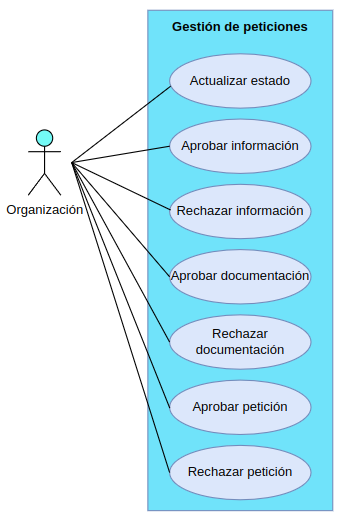
\includegraphics[width=0.8\textwidth]{imgs/gestion-peticiones}
    \caption{Gestión de peticiones}
    \label{fig:diagrama-caso-uso-gestion-peticiones}
\end{figure}

\subsubsection{Caso de Uso 3.1: Actualizar estado}\label{subsubsec:actualizar-estado-peticion}

\begin{table}[H]
    \begin{center}
        \begin{adjustbox}{width=\textwidth}
            \begin{tabular}{ | l | l | l | l | c | c | }
                \hline
                \textbf{Caso de uso} & \multicolumn{4}{l|}{Actualizar estado} & \cellcolor{gray!50} \textbf{CU-1.12}\\
                \hline
                \textbf{Actores} & \multicolumn{5}{p{0.5\linewidth}|}{Organización} \\
                \hline
                \textbf{Tipo} & \multicolumn{5}{l|}{Primario y esencial} \\
                \hline
                \textbf{Referencias} & \multicolumn{3}{l|}{RF-3.1} & \multicolumn{2}{l|}{ }\\
                \hline
                \textbf{Precondición} & \multicolumn{5}{l|}{La petición debe estar registrada en la plataforma previamente} \\
                \hline
                \textbf{Postcondición} & \multicolumn{5}{l|}{La organización actualiza el estado de una petición de la plataforma} \\
                \hline
                \textbf{Autor} & \multicolumn{1}{p{0.25\linewidth}|}{Manuel Ángel Rodríguez Segura} & \textbf{Fecha} &
                08-04-2023     & \textbf{Versión}                                                      & 1.0\\
                \hline
            \end{tabular}
        \end{adjustbox}
        \caption{CU-3.1: Actualizar estado}
        \label{tab:actualizar-estado}
    \end{center}
\end{table}

\begin{table}[H]
    \centering
    \begin{tabularx}{\textwidth}{@{} |L |@{}} \hline
        \rowcolor{gray!50}
        \textbf{Propósito} \\
        \hline
        Permite a una organización actualizar el estado de una petición de la plataforma. \\
        \hline
    \end{tabularx}
\end{table}

\begin{table}[H]
    \centering
    \begin{tabularx}{\textwidth}{@{} |L |@{}} \hline
        \rowcolor{gray!50}
        \textbf{Resumen} \\
        \hline
        Permite a una organización actualizar el estado de una petición que se haya realizado en la aplicación para
    que el usuario cuente con la información más reciente. \\
        \hline
    \end{tabularx}
\end{table}

\subsubsection{Caso de Uso 3.2: Eliminar petición}\label{subsubsec:eliminar-peticion}

\begin{table}[H]
    \begin{center}
        \begin{adjustbox}{width=\textwidth}
            \begin{tabular}{ | l | l | l | l | c | c | }
                \hline
                \textbf{Caso de uso} & \multicolumn{4}{l|}{Aprobar información} & \cellcolor{gray!50} \textbf{CU-1.13}\\
                \hline
                \textbf{Actores} & \multicolumn{5}{p{0.5\linewidth}|}{Organización} \\
                \hline
                \textbf{Tipo} & \multicolumn{5}{l|}{Primario y esencial} \\
                \hline
                \textbf{Referencias} & \multicolumn{3}{l|}{RF-3.2} & \multicolumn{2}{l|}{ }\\
                \hline
                \textbf{Precondición} & \multicolumn{5}{l|}{La petición debe estar registrada en la plataforma previamente
                y la información no puede estar rechazada} \\
                \hline
                \textbf{Postcondición} & \multicolumn{5}{l|}{La organización aprueba la información de una petición de la plataforma} \\
                \hline
                \textbf{Autor} & \multicolumn{1}{p{0.25\linewidth}|}{Manuel Ángel Rodríguez Segura} & \textbf{Fecha} &
                08-04-2023     & \textbf{Versión}                                                      & 1.0\\
                \hline
            \end{tabular}
        \end{adjustbox}
        \caption{CU-3.2: Aprobar información}
        \label{tab:aprobar-informacion}
    \end{center}
\end{table}

\newpage

\begin{table}[H]
    \centering
    \begin{tabularx}{\textwidth}{@{} |L |@{}} \hline
        \rowcolor{gray!50}
        \textbf{Propósito} \\
        \hline
        Permite a una organización aprobar la información de una petición de la plataforma. \\
        \hline
    \end{tabularx}
\end{table}

\begin{table}[H]
    \centering
    \begin{tabularx}{\textwidth}{@{} |L |@{}} \hline
        \rowcolor{gray!50}
        \textbf{Resumen} \\
        \hline
        Permite a una organización aprobar la información que ha proporcionado un usuario en una petición que se haya
    realizado en la aplicación previamente. \\
        \hline
    \end{tabularx}
\end{table}

\subsubsection{Caso de Uso 3.3: Rechazar información}\label{subsubsec:rechazar-informacion}

\begin{table}[H]
    \begin{center}
        \begin{adjustbox}{width=\textwidth}
            \begin{tabular}{ | l | l | l | l | c | c | }
                \hline
                \textbf{Caso de uso} & \multicolumn{4}{l|}{Rechazar información} & \cellcolor{gray!50} \textbf{CU-1.14}\\
                \hline
                \textbf{Actores} & \multicolumn{5}{p{0.5\linewidth}|}{Organización} \\
                \hline
                \textbf{Tipo} & \multicolumn{5}{l|}{Primario y esencial} \\
                \hline
                \textbf{Referencias} & \multicolumn{3}{l|}{RF-3.3} & \multicolumn{2}{l|}{ }\\
                \hline
                \textbf{Precondición} & \multicolumn{5}{l|}{La petición debe estar registrada en la plataforma previamente y
                la información no puede estar aprobada} \\
                \hline
                \textbf{Postcondición} & \multicolumn{5}{l|}{La organización rechaza la información de una petición de la plataforma} \\
                \hline
                \textbf{Autor} & \multicolumn{1}{p{0.25\linewidth}|}{Manuel Ángel Rodríguez Segura} & \textbf{Fecha} &
                08-04-2023     & \textbf{Versión}                                                      & 1.0\\
                \hline
            \end{tabular}
        \end{adjustbox}
        \caption{CU-3.3: Rechazar información}
        \label{tab:rechazar-informacion}
    \end{center}
\end{table}

\begin{table}[H]
    \centering
    \begin{tabularx}{\textwidth}{@{} |L |@{}} \hline
        \rowcolor{gray!50}
        \textbf{Propósito} \\
        \hline
        Permite a una organización rechazar la información de una petición de la plataforma. \\
        \hline
    \end{tabularx}
\end{table}

\begin{table}[H]
    \centering
    \begin{tabularx}{\textwidth}{@{} |L |@{}} \hline
        \rowcolor{gray!50}
        \textbf{Resumen} \\
        \hline
        Permite a una organización rechazar la información que ha proporcionado un usuario en una petición que se haya
    realizado en la aplicación previamente. \\
        \hline
    \end{tabularx}
\end{table}

\newpage

\subsubsection{Caso de Uso 3.4: Aprobar documentación}\label{subsubsec:aprobar-documentacion}

\begin{table}[H]
    \begin{center}
        \begin{adjustbox}{width=\textwidth}
            \begin{tabular}{ | l | l | l | l | c | c | }
                \hline
                \textbf{Caso de uso} & \multicolumn{4}{l|}{Aprobar documentación} & \cellcolor{gray!50} \textbf{CU-1.15}\\
                \hline
                \textbf{Actores} & \multicolumn{5}{p{0.5\linewidth}|}{Organización} \\
                \hline
                \textbf{Tipo} & \multicolumn{5}{l|}{Primario y esencial} \\
                \hline
                \textbf{Referencias} & \multicolumn{3}{l|}{RF-3.4} & \multicolumn{2}{l|}{ }\\
                \hline
                \textbf{Precondición} & \multicolumn{5}{l|}{La petición debe estar registrada en la aplicación,
                el usuario debe haber enviado la documentación previamente y no puede estar rechazada} \\
                \hline
                \textbf{Postcondición} & \multicolumn{5}{l|}{La organización aprueba la documentación de una petición de la plataforma} \\
                \hline
                \textbf{Autor} & \multicolumn{1}{p{0.25\linewidth}|}{Manuel Ángel Rodríguez Segura} & \textbf{Fecha} &
                08-04-2023     & \textbf{Versión}                                                      & 1.0\\
                \hline
            \end{tabular}
        \end{adjustbox}
        \caption{CU-3.4: Aprobar documentación}
        \label{tab:aprobar-documentacion}
    \end{center}
\end{table}

\begin{table}[H]
    \centering
    \begin{tabularx}{\textwidth}{@{} |L |@{}} \hline
        \rowcolor{gray!50}
        \textbf{Propósito} \\
        \hline
        Permite a una organización aprobar la documentación que ha enviado un usuario en una petición. \\
        \hline
    \end{tabularx}
\end{table}

\begin{table}[H]
    \centering
    \begin{tabularx}{\textwidth}{@{} |L |@{}} \hline
        \rowcolor{gray!50}
        \textbf{Resumen} \\
        \hline
        Permite a una organización aprobar la documentación que ha proporcionado un usuario en una petición que se haya
    realizado en la aplicación previamente. \\
        \hline
    \end{tabularx}
\end{table}

\subsubsection{Caso de Uso 3.5: Rechazar documentación}\label{subsubsec:rechazar-documentacion}

\begin{table}[H]
    \begin{center}
        \begin{adjustbox}{width=\textwidth}
            \begin{tabular}{ | l | l | l | l | c | c | }
                \hline
                \textbf{Caso de uso} & \multicolumn{4}{l|}{Rechazar documentación} & \cellcolor{gray!50} \textbf{CU-1.16}\\
                \hline
                \textbf{Actores} & \multicolumn{5}{p{0.5\linewidth}|}{Organización} \\
                \hline
                \textbf{Tipo} & \multicolumn{5}{l|}{Primario y esencial} \\
                \hline
                \textbf{Referencias} & \multicolumn{3}{l|}{RF-3.5} & \multicolumn{2}{l|}{ }\\
                \hline
                \textbf{Precondición} & \multicolumn{5}{l|}{La petición debe estar registrada en la aplicación,
                el usuario debe haber enviado la documentación previamente y no puede estar aprobada.} \\
                \hline
                \textbf{Postcondición} & \multicolumn{5}{l|}{La organización rechaza la documentación de una petición de la plataforma} \\
                \hline
                \textbf{Autor} & \multicolumn{1}{p{0.25\linewidth}|}{Manuel Ángel Rodríguez Segura} & \textbf{Fecha} &
                08-04-2023     & \textbf{Versión}                                                      & 1.0\\
                \hline
            \end{tabular}
        \end{adjustbox}
        \caption{CU-3.5: Rechazar documentación}
        \label{tab:rechazar-documentacion}
    \end{center}
\end{table}

\begin{table}[H]
    \centering
    \begin{tabularx}{\textwidth}{@{} |L |@{}} \hline
        \rowcolor{gray!50}
        \textbf{Propósito} \\
        \hline
        Permite a una organización rechazar la documentación que ha enviado un usuario en una petición. \\
        \hline
    \end{tabularx}
\end{table}

\begin{table}[H]
    \centering
    \begin{tabularx}{\textwidth}{@{} |L |@{}} \hline
        \rowcolor{gray!50}
        \textbf{Resumen} \\
        \hline
        Permite a una organización rechazar la documentación que ha proporcionado un usuario en una petición que se haya
    realizado en la aplicación previamente. \\
        \hline
    \end{tabularx}
\end{table}

\subsubsection{Caso de Uso 3.6: Aprobar petición}\label{subsubsec:aprobar-peticion}

\begin{table}[H]
    \begin{center}
        \begin{adjustbox}{width=\textwidth}
            \begin{tabular}{ | l | l | l | l | c | c | }
                \hline
                \textbf{Caso de uso} & \multicolumn{4}{l|}{Aprobar petición} & \cellcolor{gray!50} \textbf{CU-1.17}\\
                \hline
                \textbf{Actores} & \multicolumn{5}{p{0.5\linewidth}|}{Organización} \\
                \hline
                \textbf{Tipo} & \multicolumn{5}{l|}{Primario y esencial} \\
                \hline
                \textbf{Referencias} & \multicolumn{3}{l|}{RF-3.6} & \multicolumn{2}{l|}{ }\\
                \hline
                \textbf{Precondición} & \multicolumn{5}{l|}{La petición debe estar registrada en la aplicación y
                la información y documentación del usuario deben estar aprobadas previamente} \\
                \hline
                \textbf{Postcondición} & \multicolumn{5}{l|}{La organización aprueba la petición de la plataforma} \\
                \hline
                \textbf{Autor} & \multicolumn{1}{p{0.25\linewidth}|}{Manuel Ángel Rodríguez Segura} & \textbf{Fecha} &
                08-04-2023     & \textbf{Versión}                                                      & 1.0\\
                \hline
            \end{tabular}
        \end{adjustbox}
        \caption{CU-3.6: Aprobar petición}
        \label{tab:aprobar-peticion}
    \end{center}
\end{table}

\begin{table}[H]
    \centering
    \begin{tabularx}{\textwidth}{@{} |L |@{}} \hline
        \rowcolor{gray!50}
        \textbf{Propósito} \\
        \hline
        Permite a una organización aprobar una petición. \\
        \hline
    \end{tabularx}
\end{table}

\begin{table}[H]
    \centering
    \begin{tabularx}{\textwidth}{@{} |L |@{}} \hline
        \rowcolor{gray!50}
        \textbf{Resumen} \\
        \hline
        Permite a una organización aprobar una petición que se haya realizado en la aplicación previamente. \\
        \hline
    \end{tabularx}
\end{table}

\subsubsection{Caso de Uso 3.7: Rechazar petición}\label{subsubsec:rechazar-peticion}

\begin{table}[H]
    \begin{center}
        \begin{adjustbox}{width=\textwidth}
            \begin{tabular}{ | l | l | l | l | c | c | }
                \hline
                \textbf{Caso de uso} & \multicolumn{4}{l|}{Rechazar petición} & \cellcolor{gray!50} \textbf{CU-1.18}\\
                \hline
                \textbf{Actores} & \multicolumn{5}{p{0.5\linewidth}|}{Organización} \\
                \hline
                \textbf{Tipo} & \multicolumn{5}{l|}{Primario y esencial} \\
                \hline
                \textbf{Referencias} & \multicolumn{3}{l|}{RF-3.7} & \multicolumn{2}{l|}{ }\\
                \hline
                \textbf{Precondición} & \multicolumn{5}{l|}{La petición debe estar registrada en la aplicación previamente} \\
                \hline
                \textbf{Postcondición} & \multicolumn{5}{l|}{La organización rechaza la petición de la plataforma} \\
                \hline
                \textbf{Autor} & \multicolumn{1}{p{0.25\linewidth}|}{Manuel Ángel Rodríguez Segura} & \textbf{Fecha} &
                08-04-2023     & \textbf{Versión}                                                      & 1.0\\
                \hline
            \end{tabular}
        \end{adjustbox}
        \caption{CU-3.7: Rechazar petición}
        \label{tab:rechazar-peticion}
    \end{center}
\end{table}

\begin{table}[H]
    \centering
    \begin{tabularx}{\textwidth}{@{} |L |@{}} \hline
        \rowcolor{gray!50}
        \textbf{Propósito} \\
        \hline
        Permite a una organización rechazar una petición. \\
        \hline
    \end{tabularx}
\end{table}

\begin{table}[H]
    \centering
    \begin{tabularx}{\textwidth}{@{} |L |@{}} \hline
        \rowcolor{gray!50}
        \textbf{Resumen} \\
        \hline
        Permite a una organización rechazar una petición que se haya realizado en la aplicación previamente. \\
        \hline
    \end{tabularx}
\end{table}

Para entender de forma gráfica cómo funciona el flujo de una petición de adopción desde que se crea por el usuario hasta que se acepta
por parte de la organización, se puede consultar la siguiente figura: \\

\begin{figure}[H]
    \centering
    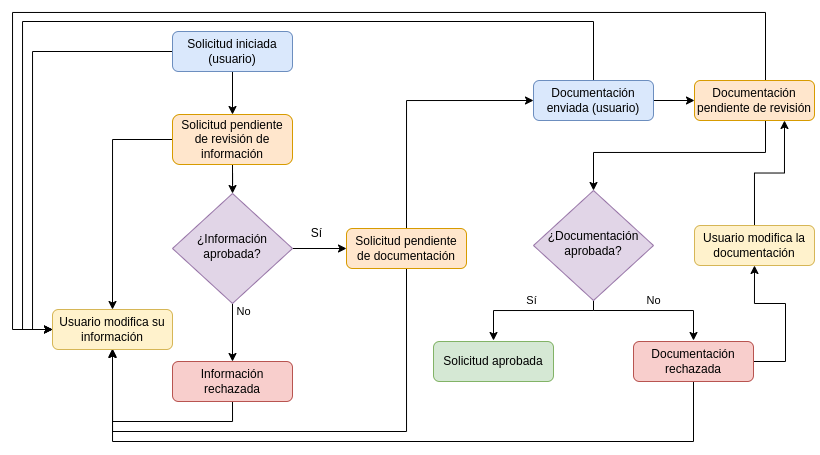
\includegraphics[width=1.0\textwidth]{imgs/estados-peticion.png}
    \caption{Flujo de una petición de adopción}
    \label{fig:flujo-peticion}
\end{figure}